%
\documentclass[12pt]{article}

% The usual packages
\usepackage{fullpage}
\usepackage{breakcites}
\usepackage{setspace}
\usepackage{endnotes}
\usepackage{float}
\usepackage{amsmath}
\usepackage{amsfonts}
\usepackage{amssymb}
\usepackage{rotating}
\usepackage{dcolumn}
\usepackage{longtable}
\usepackage{microtype}
\usepackage{graphicx}
\usepackage{hyperref}
%\usepackage[usenames,dvipsnames]{color}
\usepackage{url}
\usepackage{natbib}
\usepackage{framed}
\usepackage{epigraph}
\usepackage{lipsum}
\usepackage[font=small,labelfont=sc]{caption}
\restylefloat{table}
\bibpunct{(}{)}{;}{a}{}{,}

% Set paragraph spacing the way I like
\parskip=0pt
\parindent=20pt

% Define mathematical results
\newtheorem{lemma}{Lemma}
\newtheorem{proposition}{Proposition}
\newtheorem{theorem}{Theorem}
\newtheorem{claim}{Claim}
\newenvironment{proof}[1][Proof]{\begin{trivlist}
\item[\hskip \labelsep {\bfseries #1}]}{\end{trivlist}}
\newenvironment{definition}[1][Definition]{\begin{trivlist}
\item[\hskip \labelsep {\bfseries #1}]}{\end{trivlist}}
\newenvironment{example}[1][Example]{\begin{trivlist}
\item[\hskip \labelsep {\bfseries #1}]}{\end{trivlist}}
\newenvironment{remark}[1][Remark]{\begin{trivlist}
\item[\hskip \labelsep {\bfseries #1}]}{\end{trivlist}}

% Set up fonts the way I like
\usepackage{tgpagella}
\usepackage[T1]{fontenc}
\usepackage[bitstream-charter]{mathdesign}

%% Set up lists the way I like
% Redefine the first level
\renewcommand{\theenumi}{\arabic{enumi}.}
\renewcommand{\labelenumi}{\theenumi}
% Redefine the second level
\renewcommand{\theenumii}{\alph{enumii}.}
\renewcommand{\labelenumii}{\theenumii}
% Redefine the third level
\renewcommand{\theenumiii}{\roman{enumiii}.}
\renewcommand{\labelenumiii}{\theenumiii}
% Redefine the fourth level
\renewcommand{\theenumiv}{\Alph{enumiv}.}
\renewcommand{\labelenumiv}{\theenumiv}
% Eliminate spacing around lists
\usepackage{enumitem}
\setlist{nolistsep}

% Create footnote command so that my name
% has an asterisk rather than a one.
\long\def\symbolfootnote[#1]#2{\begingroup%
\def\thefootnote{\fnsymbol{footnote}}\footnote[#1]{#2}\endgroup}

\hypersetup{
 pdftitle={Meaningful Inferences}, % title
 pdfauthor={Kelly McCaskey and Carlisle Rainey}, % author
 pdfkeywords={hypothesis testing} {confidence intervals} {substantive significance}
 pdfnewwindow=true, % links in new window
 colorlinks=true, % false: boxed links; true: colored links
 linkcolor=red, % color of internal links
 citecolor=red, % color of links to bibliography
 filecolor=red, % color of file links
 urlcolor=red % color of external links
}

% enable comments in pdf
\newcommand{\kelly}[1]{\textcolor{blue}{#1}}
\newcommand{\carlisle}[1]{\textcolor{magenta}{#1}}


\begin{document}

\begin{center}
{\LARGE Meaningful Inferences}\\\vspace{2mm}
{\large The Importance of Explicit Statistical Arguments for Substantive Significance\symbolfootnote[1]{We thank [many people]. The analyses presented here were conducted with \texttt{R} 3.1.0 and Stata 13. All data and computer code necessary for replication are available at \href{https://github.com/carlislerainey/meaningful-inferences}{github.com/carlislerainey/meaningful-inferences}.}}\\\vspace{2mm}


\vspace{10mm}

\kelly{Kelly McCaskey}\symbolfootnote[2]{Kelly McCaskey is a Ph.D. student in the Department of Political Science, University at Buffalo, SUNY, 520 Park Hall, Buffalo, NY 14260 (\href{mailto:kellymcc@buffalo.edu}{kellymcc@buffalo.edu}).}

\vspace{3mm}

\carlisle{Carlisle Rainey}\symbolfootnote[3]{Carlisle Rainey is Assistant Professor of Political Science, University at Buffalo, SUNY, 520 Park Hall, Buffalo, NY 14260 (\href{mailto:rcrainey@buffalo.edu}{rcrainey@buffalo.edu}).}
\end{center}

% Remove page number from first page
%\thispagestyle{empty}

\vspace{10mm}



% Abstract
{\centerline{\textbf{Abstract}}}
\begin{quote}\noindent
Research political science is gradually moving away from an exclusive focus on statistical significance testing and toward an emphasis of effect magnitude. We argue that the current practice of ``magnitude-and-significance'' is only a small improvement over the much maligned ``sign-and-significance'' approach to interpreting statistical results. We argue that instead of interpreting the magnitude of statistically significant effect, researchers should explicitly account for uncertainty when making judgments about substantive significance. This requires the researcher to precisely defined the effects that are substantively meaningful and show that those effects are unlikely to generate the observed data. We use to replications of published work to illustrate our suggested approach.
 \end{quote}
\thispagestyle{empty}

%\epigraph{Data analysis must use mathematical argument and mathematical results as bases for judgment rather than as bases for proof or stamps of validity.}{Tukey (1962, p. 6)}
\epigraph{Far better an approximate answer to the \textit{right} question, which is often vague, than an exact answer to the \textit{wrong} question, which can always be made precise.}{Tukey (1962, p. 13-14)}
%\epigraph{...an investigator would be misled less frequently and would be more likely to obtain the information he seeks were he to formulate his experimental problems in terms of the estimation of population parameters, with the establishment of confidence intervals about the estimated values, rather than in terms of a null hypothesis against all possible alternatives.}{Lyle V. Jones (1955, p.407)}
%\epigraph{Tests of significance are preliminary or ancillary. The emphasis on tests of significance, and the consideration of the results of each experiment in isolation, have had the unfortunate consequence that scientific works have regarded the execution of a test of significance on an experiment as the ultimate objective. Results are significant or not significant and that is the end of it.}{Yates (1951, p. ???)}

%\end{document} % uncomment to make a title-page with author info

\newpage
\doublespace
% Set first page of text as page 1. I don't care for this
%   feature because then the page numbers don't correspond
%   to the pdf pages.
%\setcounter{page}{1}

\section*{Introduction}

\carlisle{[Introduction here.--Write later.]}

\section*{What We Want To Know}

\kelly{[It would be great to have a running example throughout this section. Perhaps a recent paper goes through these steps in a clear manner and we could briefly describe what the authors do. I'm sure that lots of papers do it, but it might be hard to find a clear, simple example that doesn't require too much background. \textbf{We just need an example of an effect (from a published paper) about which we'd like to ask the three questions below. It doesn't matter if the authors answer them or not.}]}

Most empirical research in political science focuses on estimating the effect $\Delta$ of an explanatory variable $x$ on the expected value of an outcome of interest $y$. Formally, we might suppose that $E(y | x) = f(x)$ and define the ``effect'' or ``quantity of interest'' $\Delta$ as the difference between the average outcomes when $x$ takes on a substantively meaningful high value and low value, so that $\Delta = E(y | x = x_{hi}) - E(y | x = x_{lo}) = f(x_{hi}) - f(x_{lo})$. Importantly, empirical work usually focuses on answering three fundamental questions about the effect $\Delta$ of $x$ on $y$. 

\begin{enumerate}
\item What is the direction of the effect?
\item How large is the effect?
\item Is the effect substantively important?
\end{enumerate}

Each of these question requires increasing levels of analysis and substantive interpretation and each receives decreasing levels of attention in political science research. From 2011 to 2013, both APSR and AJPS published a total of 316 total articles, 73\% of which were empirical analyses. Of this 73\%, approximately half of the articles discuss finding substantively meaningful results while the other half do not. Furthermore, of the articles that discuss their substantively meaningful results, only 17\% provide an argument as to the importance of the substantive interpretation.

\subsection*{Establish the Sign}

The first question that question that empirical research usually attempts to answer is the direction of the effect. Is the effect positive or negative?\footnote{Some research argues theoretically and empirically for ``no effect'' or ``a negligible effect'' (e.g., Kam and Palmer 2008, see Rainey 2014), but most hypotheses posit the direction of an effect.} For instance, Wilson and Piazza (2013) hypothesize that ``democratic regimes are more likely to experience terrorism," (945) while Gamm and Kousser (2013) posit that ``as the size of the city's delegation in the legislature (logged) increases, passage rates of that city's district bills will fall, ceteris paribus," (668). 

Suppose, for clarity, that the researcher offers a directional research hypothesis, suggesting that an effect of interest $\Delta$ is positive. Formally, we might denote this hypothesis as $H_r: \Delta > 0$. Then the researcher compares this research hypothesis to a null hypothesis that suggests that the research hypothesis is false, or equivalently, that the effect lies outside the region suggested by the research hypothesis. Formally, we might write this as $H_0: \Delta \leq 0$. To assess the evidence against the null hypothesis, the researcher usually calculates a $p$-value, which is the probability of obtaining (hypothetical) data at least as extreme as the observed data if the null hypothesis were true.\footnote{This is always the case in our sample.} If this $p$-value is sufficiently small (by convention, less than 0.05), then the researcher rejects the null hypothesis in favor of the research hypothesis. In our example, the researcher would reject negative effects and conclude that the effect is positive. However, if the $p$-value is not sufficiently small, then the researcher declares that the data do not offer compelling evidence against the null and notes that the direction of the effect remains uncertain.\footnote{However, some research takes a $p$-value greater than 0.05 as evidence \textit{in favor of} the null hypothesis (Rainey 2014). We prefer to interpret a lack of statistical significance as ambiguous evidence from which the researcher can make no claim (i.e., the effect might be negative or positive). In this sense, a Type-II (i.e., false-negative) error is not so much of an error as a lost opportunity (Tukey 1991).}

Broockman (2013) provides an example of this ``sign-and-significance" approach. He conducts a field experiment to test his hypothesis that black legislators are significantly more intrinsically motivated to contribute to the black community. When evaluating his empirical results, Broockman is able to reject the null hypothesis based on its $p$-value being sufficiently small, deeming the results as statistically significant. 

\kelly{[The sign-and-significance approach is really just a matter of emphasis--emphasizing statistical significance over magnitude of effects. Is there any way we can use quotes from Broockman to illustrate this?]}

There are three aspects of the sign-and-significance approach make note of. First, this style of argumentation is ubiquitous in political science. It is extremely rare to find empirical research in political science that does not perform a hypothesis test of some sort. Each and every empirical study in our sample performed some type of hypothesis test. Second, note that this approach is compelling not because it argues that the observed data are consistent with the researcher's claim, but because the data are inconsistent with other claims. Third, notice that this argument for the direction of the effect explicitly takes into account the uncertainty of the estimated effect. If the uncertainty is large relative to the magnitude of the estimate then the researcher cannot (and usually does not) make confident claims about the direction of the effect of interest. \kelly{[We could put a really nice example here of a researcher drawing a cautious conclusion from an insignificant effect.]} However, if the uncertainty is small relative to the size of the estimated effect, then the researcher can draw confident conclusions about the direction of the effect. \kelly{[We could put a really nice example here of a researcher drawing a confidence conclusion from a significant effect.]}

\subsection*{Establish the Magnitude}

Yet recent methodological work emphasizes that empirical work should go beyond estimating the direction of the effect (King, Tomz, Wittenberg 2000; Hanmer and Kalkan 2013; Gross 2014). In addition to the direction of an effect, the size of the effect matters as well. 

Some statistical models have parameters that are naturally interpretable. For example, a simple difference-in-means or normal-linear model have directly interpretable coefficients as long as the scales of the variables are reasonable and the model does not include non-linear or product terms. Outside of these atypical situations, however, the researcher must do additional work to estimate a substantively meaningful quantity of interest.

In discussing how scholars might interpret a model of the effects of education on income, King, Tomz, and Wittenberg (2000, p. 348) write:

\begin{quote}
Bad interpretations are substantively ambiguous and filled with methodological jargon: `the coefficient on education was statistically significant at the 0.05 level.' Descriptions like this are very common in social science, but students, public officials, and scholars should not need to understand phrases like `coefficient,' `statistically significant,' and `the 0.05 level' to learn from the research. Moreover, even statistically savvy readers should complain that the sentences does not convey the key quantity of interest: how much higher the starting salary would be if the student attended college for an extra year.
\end{quote}

The emphasis on effect magnitude is not a new idea. Commenting on the consequences of Fisher's null hypothesis significance test, Yates (1951, ???) writes: ``[I]t has caused scientific workers to pay undue attention to the results of the tests of significance they perform on their data, particularly data derived from experiments, and too little to the estimates of the magnitude of the effects they are investigating.'' Yates continues: 

\begin{quote}
Tests of significance are preliminary or ancillary. The emphasis on tests of significance, and the consideration of the results of each experiment in isolation, have had the unfortunate consequence that scientific works have regarded the execution of a test of significance on an experiment as the ultimate objective. Results are significant or not significant and that is the end of it (???).
\end{quote}

Fortunately, recent conceptual work (King, Tomz, and Wittenberg 2000; Berry, DeMeritt, and Esarey 2010; and Hanmer and Kalkan 2013) and software development (Tomz, Wittenberg, King 2003; Imai, King, Lau 2007) empowers political scientists to move beyond a simple ``sign-and-significance'' approach and also present substantively meaningful measures of effect magnitude. Cohen (2013), Flores-Macias and Kreps (2013), and Kastellec (2013), with the use of Tomz, Wittenberg and King's CLARIFY, all employ first-differences to determine substantively meaningful effect sizes.

\kelly{[Again, we need to illustrate this with quotes.]}

\subsection*{Establish the Substantive Importance}

But ultimately, researchers want to move beyond the simple presentation of effect magnitude and make a judgment about the meaningfulness of the effects. Is the effect large or small? Is it substantively important? Is it relevant for policy? Is it scientifically important? Is it large enough to matter? Hanmer and Kalkan (2013, p. 264) write: ``[W]e take it as given that understanding whether the relationship is substantively significant, rather than just statistically significant, is the ultimate goal, as it is a necessary part of vaulting one's theory.''

\carlisle{[Add something here about what makes something substantively important.]}

For example, Kinne (2013) presents substantively meaningful effects that are substantively large enough to be important. He hypothesizes that there are three discernible ways that states network and form bilateral agreements and determines whether or not these are both statistically and substantively significant through his empirical analysis. By determining which effects are substantively meaningful, he is able to make the claim that his research makes a substantial contribution to the literature on international cooperation. 

\kelly{[We need some quotes here. How does Kinne make the claim that the estimates are substantively meaningful? Does he just assert it?]}

\section*{Potential Pitfalls in Reasoning About Effect Magnitude}

There are two possible errors that researchers might make when making claims about the substantive magnitude of the effect. The first potential mistake that researchers might make is interpreting the $p$-value as a measure of magnitude or importance (e.g., Cohen 1990 and Gill 1999).

The second potential pitfall is interpreting the magnitude without explicitly accounting for the uncertainty of the estimate. This mistake is more subtle, but has negative consequences that are nearly as severe as the first. 

\subsection*{Small $p$-Values Do Not Indicate Large Effect}

A $p$-value is simply the probability of observing data at least as extreme as the observed data if the null hypothesis were true (e.g., Casella and Berger 2002 and DeGroot and Schervish 2002). All else equal, the $p$-value gets smaller as the effect size under investigation increases, but the $p$-value is also a function of the sample size (Gill 1999). While it is common to describe estimates as ``highly significant'' or ``very significant,'' this implies (or tempts readers to conclude) that an effect is large or important. However, a minuscule $p$-value does not imply a large or important effect. ``Very significant'' (e.g., $p < 0.001$) might simply mean that the researcher has a large sample. Even if the researcher finds statistically significant results with a small sample, the small $p$-value only indicates that the effect size is large relative to the uncertainty. It says nothing about the size of the estimate relative to some standard of substantive importance. With a very small $p$-value (e.g., $p < 0.001$), substantive experts might judge the effect to be large, moderate, small, or even negligible. Experts might call some of these effect important, somewhat important, slightly important, or not at all important. The $p$-value is indirectly related to substantive significance at best. This disconnect occurs for two reasons. First, the $p$-value is only partly determined by the effect size--sample size plays a large part as well. Second, the absolute magnitude of the effect cannot be deemed substantively large, small, or negligible without the judgment of a substantive expert.

\subsection*{Current Practice Does Not Account for Uncertainty}

The standard scientific practice in political science computes substantively interpretable estimates of effects and (1) determines whether these estimates are statistically significant and, if so, (2) makes a judgement about whether the magnitude is substantively important. \kelly{[We need to add a cite here, but perhaps several examples will do. I'm confidence that this is the way it is done in practice, but we need to either point to a source that suggests the practice or illustrate with several examples that the practice is quite common.]} This two step procedure has three unfortunate consequences. This tempts researchers to...
\singlespace
\begin{enumerate}
\item treat all results that are not statistically significant similarly, drawing no distinction between large, imprecise estimates and small, precise estimates (see Rainey 2014).
\item treat all statistically significant and substantively large estimates similarly, drawing no distinction between large, imprecise estimates and large, precise estimates.
\item treat ``barely significant,'' large estimates and ``almost significant,'' large estimates quite differently, drawing a strong distinction between two similar estimates with similar uncertainty.
\end{enumerate}
\doublespace

Consider, for example the hypothetical studies presented in Figure \ref{fig:example-cis}. If we considered 0.25 the minimal substantively meaningful effect, then only one study, Study A, seems to offer evidence for a substantively meaningful effect. Yet the current practice would also suggest that Study B offers evidence for a substantively meaningful effect as well. And while a large, meaningful effect is certainly plausible based on Study B, it fails to rule out small, negligible effects. In fact, the amount of evidence offers for the hypothesis of a meaningful effect by Study B is similar to that offered by Study C--neither study rules our small, negligible effects. Yet these studies are treated quite differently by the current practice in political science. In fact, the only improvement of the current practice over the sign-and-significance method is that the current practice managed to distinguish between Study D and Study A.

\begin{figure}[h]
\begin{center}
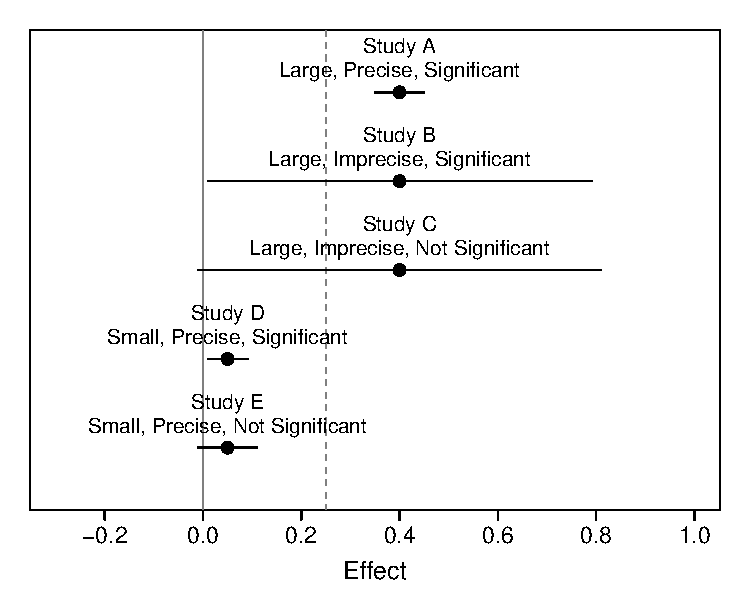
\includegraphics[scale = .6]{figs/example-cis.pdf}
\caption{This figure provides several hypothetical studies to illustrate several points about arguments for substantive significance. Notice that Studies D and E produce similar results and Studies B and C produce similar estimates. If we take 0.25 as a the smallest substantively meaningful effect, then only Study A offers compelling evidence for a meaningful effect. Unfortunately, the current practice treats Studies A and B (and perhaps D) as similar evidence for a meaningful effect. See Table \ref{tab:example-cis} for the typical interpretations.}\label{fig:example-cis}
\end{center}
\end{figure}

\renewcommand{\arraystretch}{1.5}
\begin{table}
\begin{center}
\begin{scriptsize}
\begin{tabular}{|>{\centering\arraybackslash}m{.5in}>{\centering\arraybackslash}m{1.75in}>{\centering\arraybackslash}m{1.75in}>{\centering\arraybackslash}
m{1.75in}|}
\hline

Study & Sign and Significance Method & Current Practice & Intuitive Interpretation\\ 
\hline
Study A & ``positive and significant'' & ``positive, significant, and substantively large'' & ``We have strong evidence for a large, substantively meaningful effect.''\\
Study B & ``positive and significant'' & ``positive, significant, and substantively large'' & ``We have only weak evidence for a large, substantively meaningful effect, because the data are also consistent with negligible effects near zero.''\\
Study C & ``not statistically significant'' & ``not statistically significant'' & ``We have only weak evidence for a large, substantively meaningful effect, because the data are also consistent with negligible effects near zero.''\\
Study D & ``positive and significant'' & ``positive and significant, but substantively small' & ``We have strong evidence against a substantively meaningful effect.''\\
Study E & ``not statistically significant'' & ``not statistically significant'' & ``We have strong evidence against a substantively meaningful effect.''\\
\hline
\end{tabular}\caption{This table provides the typical interpretations of the results in Figure \ref{fig:example-cis} using the two common methods. Notice that the sign-and-significance methods and the current practice only manage to distinguish the evidence from Studies D and E. The current practice treats Studies A and B similarly and Studies C and E similarly. However, these studies offer vastly different amounts of evidence for or against an hypothesis of a meaningful effect.}\label{tab:example-cis}
\end{scriptsize}
\end{center}
\end{table}

The key takeaway point is that it is important to apply similar standards of evidence to arguments for positive (or negative) effects and arguments for meaningfully positive (or meaningfully negative) effects. The usual logic of hypothesis testing requires that the researcher only declare that an effect is positive if and only if the evidence points overwhelming against negative effects. Similarly, researchers should not declare a positive estimate substantively meaningful simply because it is inconsistent with with negative effects and above some threshold. A better standard of evidence would require that researchers declare an effect meaningful if and only if it is inconsistent with negligible effects.



\section*{A Compelling Argument for a Meaningful Effect}

Researchers can make much more compelling and transparent arguments for meaningful effects by explicitly testing the claims we are making. For example, if  a researcher claims that an effect is positive and substantively meaningful, then the research hypothesis is not $H_r: \Delta > 0$. Instead, it's $H_r: \Delta > m$, where $m$ represents the researchers judgment about the smallest substantively interesting effect (or the largest substantively negligible effect). There is no need to jettison the entire hypothesis testing framework. In fact, the problems identified above can be addressed and the usual hypothesis testing framework can be kept intact if researchers are simply willing to apply their substantive judgment about which effects are and are not meaningful to their hypotheses rather than the estimated magnitude. 

The current practice in political science for arguing for a meaningful effect proceeds as follows:

\singlespace
\begin{enumerate}
\item Hypothesize that an effect is positive (or negative).
\item Test the hypothesis by computing a $p$-value. 
\item If the null hypothesis can be rejected (i.e., $p < 0.05$), then claim support for the hypothesis and compute a substantively interpretable measure of the estimated effect size and make a substantive judgment about whether the estimate is substantively meaningful or not. If the null hypothesis cannot be rejected (i.e., $p < 0.05$), then note that the evidence is unclear and do not interpret the magnitude of the estimate.
\end{enumerate}
\doublespace

The alternative approach that we propose proceeds as follows:
\singlespace
\begin{enumerate}
\item Hypothesize that the effect is positive and substantively meaningful (or negative and substantively meaningful).
\item Make a substantive judgment about the smallest substantively meaningful effect. That is, choose an $m$ such that $m$ represents the smallest substantively meaningful effect.
\item Test the research hypothesis $H_r: \Delta > m$ using a conventional hypothesis testing approach.
\end{enumerate}

\doublespace

\subsection*{Stating a Research Hypothesis of a Meaningful Effect}

The first step is easy, but important. In order to make compelling arguments for meaningful effects, researcher must clearly state their claims. Rather than simply hypothesizing that an effect is positive or negative, researcher must make their claim that a variable has a meaningful effect from the outset. For example, Levendusky and Horowitz (2012) hypothesize that ``bipartisan support in Congress for the president's policy should decrease audience costs.'' Notice that this hypothesizes a direction, but not a magnitude of the effect. Yet in discussing this hypothesis, Levendusky and Horowitz write: 

\begin{quote}
This type of unexpected (disconfirming) cue has an especially large effect on voters' decision-making processes (Baum and Groeling 2009; Eagly, Wood, and Chaiken 1978). In effect, it sends voters a strong signal that this is not a partisan decision, but rather a decision about what is best for the nation. Further, the fact that even the president's rivals supported his decision suggests to voters that the president did make the right call, which should lead all voters (regardless of partisan affiliation) to punish the president less harshly, thereby minimizing audience costs. [italics ours]
\end{quote}

Thus, Levendusky and Horowitz carefully theorize about the magnitude of the effect, but only include the direction implied by the theory, and not the magnitude, into their hypothesis. They could improve the test of their theory by building the implication about the size of the effect directly into their hypothesis, predicting that ``bipartisan support in Congress for the president's policy should substantially decrease audience costs.'' I have simply added ``substantially'' to their hypothesis. This provides a strong indication to readers (and the researcher) that the theory implies the effect should be large and the researcher will provide a strong argument for a large negative effect, as opposed to simply a negative effect. 


\subsection*{Choosing $m$}

In order to make a compelling argument that an effect is substantively meaningful, the researcher must carefully define exactly which effects are and are not substantively meaningful. This quantity is the identical concept proposed by Rainey (2014), and as Rainey notes, political scientists should not insist on hard and fast rules for judging the effects that are and are not substantively meaningful.\footnote{We should note, though, that such rules of thumb have been presented, see Glass (1976) and Cohen (1992), but these rules are usually proposed with caution.} Instead, we must insist that substantive scholars making substantive claims about politics also make substantive judgments about the importance of their effects. Thompson (2001) notes for example, that ``if people interpreted effect sizes with the same rigidity that $\alpha = 0.05$ has been used in statistical testing, we would merely be being stupid in another metric.'' Kirk (1996) notes that this judgment is ``influenced by a variety of factors, including the researcher's value system, societal concerns, assessment of costs and benefits, and so on." Despite this element of subjectivity, Thompson (2002) writes: ``[T]he existence of effect size benchmarks should not justify abrogating the responsibility for arguing for effect import in the specific context of a given study. It is not necessary to have universal benchmarks regarding what effect sizes may be deemed noteworthy. The reader with a value system widely different than that of an author might reasonably disagree with the author about whether the effect size is noteworthy and then simply ignore the study.'' 

Formal hypothesis tests and judgments about substantive importance are qualitatively different decisions and have different strengths and weaknesses. Estimation and hypothesis tests are relatively automatic and ``objective,'' but are not at all transparent. Researchers do not fit one model and report the single $p$-value. Instead they fit many models and report the one that ``makes most sense'' in light of their approach, theoretical model, normative concerns, and the results of the model. (Gerber and Malhotra 2008; Simmons, Nelson, and Simonsohn 2011; Francis 2013; Simonsohn, Nelson, and Simmons 2013; and Esarey and Wu 2014; see also Gelman and Loken 2014). Substantive judgments about effect sizes, however, require a large initial investment of careful thought to argue that certain effects are or are not substantively important. This judgment demands subjectivity. However, this subjective judgment is quite transparent. Readers are free to reject the author's judgment and substitute their own. Further, ``automatic'' and ``objective'' procedures are not always (or perhaps usually) desirable. Substantive scholars making substantive points about politics should be allowed and encouraged to make substantive judgments about magnitude (Achen 1982). Indeed, Kirk (1996) writes:

\begin{quote}
[R]esearchers have an obligation to make this kind of judgment. No one is in a better position than the researcher who collected and analyzed the data to decide whether or not the results are trivial. It is a curious anomaly that researchers are trusted to make a variety of complex decisions in the design and execution of an experiment, hut in the name of objectivity, they are not expected or even encouraged to decide whether data are practically significant.(755).
\end{quote}

\section*{Testing a Hypothesis of a Meaningful Effect}

Once the researcher has clearly identified that set of effects that he considers substantively meaningful, the testing problem is straightforward. For an effect of interest $\Delta$, the a researcher positing a ``substantively meaningful, positive effect'' must simply test her research hypothesis $H_r: \Delta > m$ against the null hypothesis $H_0: \Delta \leq m$. For a researcher positing a ``substantively meaningful, negative effect'' must simply test her research hypothesis $H_r: \Delta < -m$ against the null hypothesis $H_0: \Delta \geq -m$.\footnote{Though rarely used in practice, this the way hypothesis testing is introduced in in introductory textbooks (e.g., Wonnacott and Wonnacott 1990).}

The case of $t$-statistics illustrates the parallel between testing for a meaningful positive effect and simply testing for a positive effect. If a researcher simply wishes to argue that an effect is positive (though perhaps substantively irrelevant), the $t$-statistic is given by $t = \dfrac{\Delta}{\sqrt{\widehat{Var}(\Delta)}}$. If a researcher wishes to argue that an effect is positive and substantively meaningful, then the required $t$-statistic is given by $t = \dfrac{\Delta - m}{\sqrt{\widehat{Var}(\Delta)}}$. The researcher can then use this $t$-statistic to compute $p$-values and determine if the respective null hypothesis of ``no effect'' or ``a negligible effect'' can be rejected.

\subsection*{Confidence Intervals}

While the hypothesis testing framework is sometimes clear and convenient, confidence intervals offer even more information and are easier for readers (and researchers) to interpret. Specifically, the researcher simply needs to check that a 90\% confidence interval contains values that are only consistent with the research hypothesis of a meaningful effect. Therefore, if the 90\% confidence interval contains only large, meaningful effects, then the researcher can confidently reject small, negligible effects. However, if the 90\% confidence interval contains effects that are inconsistent with the hypothesis of a meaningful effect, such as small, negligible effects, the evidence for the researchers claim is (correctly) identified as weaker. 

A $100(1-\alpha)$\% confidence interval contains the set of values that cannot be rejected by a size-$\alpha$ two-tailed test. Thus, all values $u^{+/-}_{\alpha}$ that fall outside (i.e., above or below) the confidence interval are rejected by a two-tailed test of size $\alpha$. Confidence intervals have a similar relationship with one-tailed tests. All values $u^{-}_{2\alpha}$ that fall \textit{below} a $100(1-2\alpha)$\% are rejected by a one-tailed test of the null hypothesis that the true parameter lies at or below $u^{-}_{2\alpha}$. Similarly, all values $u^{+}_{2\alpha}$ that fall \textit{above} a $100(1-2\alpha)$\% are rejected by a one-tailed test of the null hypothesis that the true parameter lies at or above $u^{+}_{2\alpha}$. Thus, there is a one-to-one correspondence between one- and two-tailed hypothesis tests of size $\alpha$ and 90\% and 95\% confidence intervals respectively (see esp. Casella and Berger 2002, pp. 419-423).

Concretely, if the researcher predicts that an effect is positive and finds that the 90\% confidence interval contains only positive effects, this is equivalent to rejecting the null hypothesis that the effect is less than or equal to zero at the 0.05 level.\footnote{Similarly, if the researcher predicts that an effect is \textit{negative} and finds that the 90\% confidence interval contains only \textit{negative} effects, this is equivalent to rejecting the null hypothesis that the effect is \textit{greater} than or equal to zero at the 0.05 level (see Freedman, Pisani, and Purves 2007 pp. 383-385 for more on this point and DeGroot and Schervish 2012 pp. 485-493 for an alternative perspective).}

%Thus, confidence intervals partition the parameter space into the effects that are plausible (given the data and the model) and those that are not.\footnote{Some care is warranted in interpreting confidence intervals . It is tempting for researchers to say that ``because the 90\% confidence interval ranges from 0.1 to 0.4, there is a 90\% chance that the true effect falls between 0.1 and 0'' (Hoestra, Morey, Rouder, and Wagenmakers 2014). However, frequentist confidence intervals require the probability statement to be placed on the statistic (in this case, the confidence interval) and not the parameter. Some statisticians therefore prefers the language ``we can be 95\% confidence that the true value lies between 0.1 and 0.4,'' though this requires a technical understanding of the word confident. In most applied settings, though, frequentist confidence intervals and Bayesian credible intervals, which can be interpreted as probability statements about parameters, are nearly identical (though see Berger and Wolpert 1998, ch. 2), rendering the debate somewhat moot.}

%Kirk (2001) writes:

%\begin{quote}
%A confidence interval is just as useful as a null hypothesis significance test for deciding whether chance or sampling variation is an unlikely explanation for an observed effect. Unlike a test statistic for, say, a contrast in means, a point estimate and confidence interval use the same unit of measurement as the data. This facilitates the interpretation of results and makes trivial effects harder to ignore.
%\end{quote}

\section*{Replication of Hultman, Kathman, and Shannon (2013)}

To illustrate how our approach can be used by a researcher to explicitly test their substantive claims, we replicated Hultman, Kathman, and Shannon's (2013) assessment of civilian protection by UN peacekeeping operations (PKOs). Hultman, Kathman, and Shannon offer a theory that civilians can be successfully protected by UN PKOs when those missions are composed of military troops and police in adequately large numbers. Following convention, these authors present their empirical results by (1) showing that the relevant quantity of interest is statistically significant and (2) arguing that the estimated effect is substantively meaningful.

They argue that PKOs mitigate violence both on the battlefield and behind the battlefield's frontlines for a variety of reasons while the UN's ability to intervene is contingent upon the size and personnel composition of the deployment. To evaluate this argument, Hultman, Kathman, and Shannon hypothesize that as the UN commits both more military troops and more police personnel to a conflict, the amount of violence committed against civilians will decrease. Because their original hypothesis is directional, we can use two one-tailed tests, as detailed in the previous section, to check whether or not the 90\% confidence interval contains values that are consistent only with a hypothesis of a meaningful effect. 

Noting that the relevant coefficients are statistically significant and correctly signed, Hultman, Kathman, and Shannon write:

\begin{quote}
The negative and statistically significant ($p < 0.001$) effects of \textit{UN Military Troops} and \textit{UN Police} suggest that as PKOs are increasingly supplied with soldiers and police forces, violence against civilians in civil war decreases (p. 9-10)
\end{quote}

However, following the advice of the literature on interpreting the magnitude of the effects Hultman, Kathman, and Shannon present a plots of the expected civilian deaths as the number of military and policy troops varies. We replicate these plots in Figure ??.

They write:

\begin{quote}
The figure shows that increasing the number of troops has a dramatic effect on improving the safety of noncombatants. With no troops deployed to a conflict, the expected number of civilians killed in a given month is approximately 106. When the number of UN military troops increases to 8,000, the expected value of civilian deaths declines to 1.79. Conditional on the other variables being held at the specified values, supplying only several thousand military troops nearly mutes violence completely as the number of troops approaches the upper values reported (p. 11)
\end{quote}

They argue that this reduction from an average of about 106 to about 2 is substantively important.

\begin{quote}
Bear in mind that the values presented are expected civilian deaths per month. These are not inconsequential reductions in violence. Indeed, given that the average length of a conflict in these data is nearly 65 months, deploying highly equipped missions can mitigate or wholly avert humanitarian disasters (p. 11).
\end{quote}

However, they do not explicitly take uncertainty into account when arguing for a meaningful effect. Instead, they only check that the estimate is substantively important. They do not consider whether all the plausible effects, given the data, are meaningful.

Following their use of a negative binomial model, we replicate their results, calculate second-differences, and 90\% confidence intervals around the change in the expected civilian deaths as UN military troops increases. Figure \ref{fig:hks-ci} shows these confidence intervals. At an expense of \$2 million, or roughly 2,000 troops, leads to about 65 fewer civilian casualties, on average. However, the data strongly suggest that the effect leads to \textit{at least} 45 fewer civilian casualties and possibly as many as 95. Similarly, an expense of about \$8 million, or 8,000 troops, leads to the prevention of approximately 100 civilian casualties. However, effects small than about 70 fewer civilian deaths are inconsistent with these data and the effect might be as large as 140 fewer deaths. 

In this case, the authors have strong evidence for a meaningful effect, even after uncertainty is taken into account. The authors are able to confidently reject trivial effect sizes because the confidence intervals contain only meaningful effects.

\begin{figure}[h]
\begin{center}
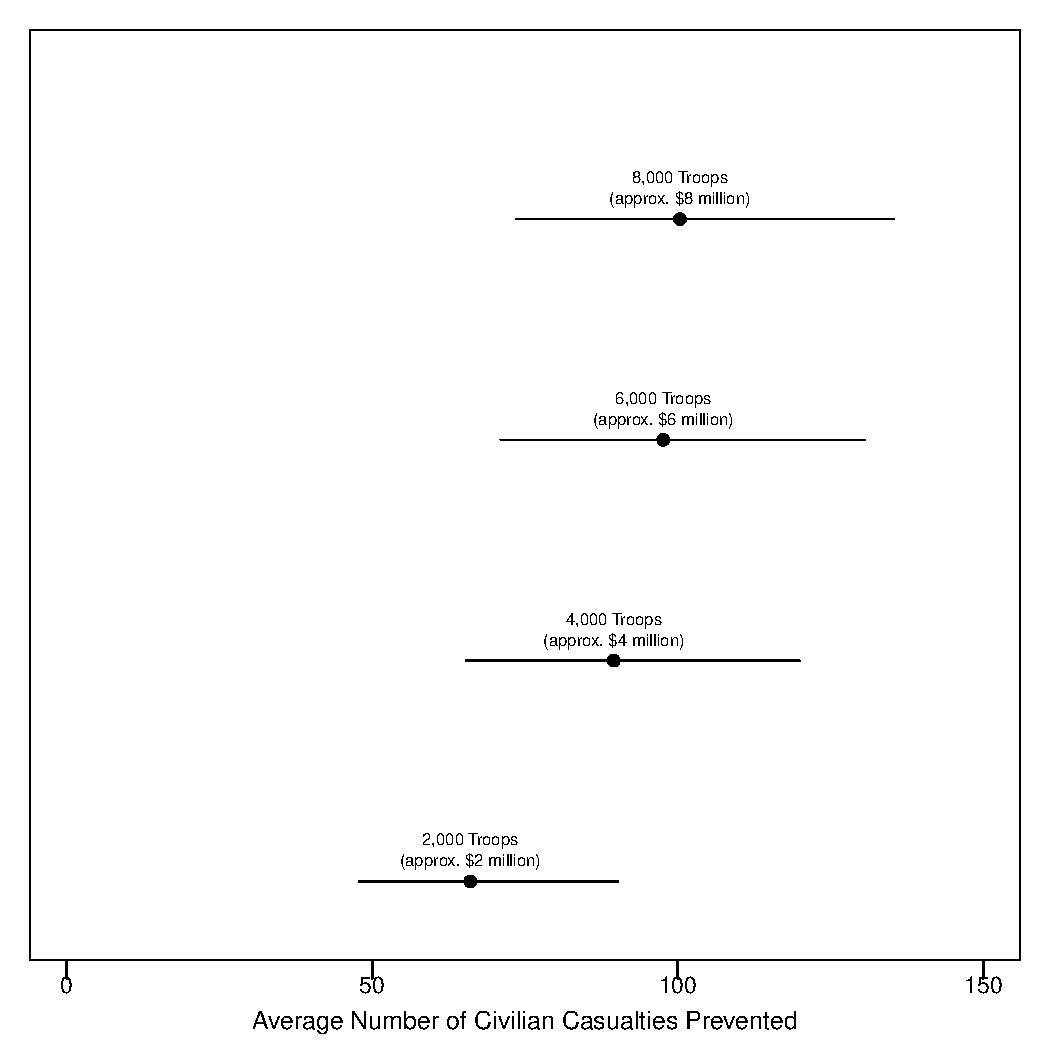
\includegraphics[scale = .8]{figs/hks-ci.pdf}
\caption{This figure provides first differences, in dollar and troop amounts, and their corresponding number of prevented civilian casualties.}\label{fig:hks-ci}
\end{center}
\end{figure}

\section*{Replication of Kam and Zechmeister (2013)}

Kam and Zechmeister (2013) argue that candidate name recognition informs voters about candidate viability.

The authors present three lab experiments to demonstrate the cause link between their concepts of interest but turn to a field experiment to boost the external validity of the results. Through a clever design exploiting routes that parent must use to drop their kids off at school, Kam and Zechmeister expose half of parents in a particular geographic region to a yard sign displaying a fictitious candidate Ben Griffin's name. The other half of parents are not exposed and serve as a control group. The authors then surveyed the parents and asked them to indicate their top three choices for city council seats by choosing among five actual candidates and two fictional candidates (one whose name appeared on yard signs and a second, placebo, whose name did not appear on any signs). The authors summarize their results:

\begin{quote}
Did recognition spurred on by political yard signs increase support for Ben Griffin in the treatment group? To determine if this is so, we examine the extent to which survey respondents selected Ben Griffin as one of their top three choices for council. As shown in [their] Table 3, in the control condition, only 13.9\% of respondents placed Ben Griffin among their top three choices, but in the treatment condition, 23.9\% of respondents placed Ben Griffin among their top three choices. This 10 percentage point difference is sizable given the modesty of the treatment. In light of the small sample size, it is statistically significant at generous levels ($p \approx 0.13$, one-tailed).
\end{quote}

But can we be confident that this effect is indeed ``sizable''? Are small effects plausible given the data?


\kelly{[Add replication here]}

\section*{Discussion}

In this paper, we have laid out an approach that allows researchers to make strong empirical arguments that effects of interest are substantively significant. However, we would like to suggests two extensions and raise a caveat.

\subsection*{Caveats}

Our goal is not to bring past research into question or to suggest that researchers should never test a simple directional hypothesis. Instead, our goal is to provide future researchers with a tool to strengthen their claims and more clearly communicate their evidence to readers in \textit{some} situations. Indeed, while testing a null hypothesis of exactly no effect has received ample criticism from methodologists (Gill 1999, Gross 2014, Hill and Jones 2014), some researchers defend its merits (e.g., Hagan 1997 and Wainer 1999 \carlisle{I might want to add Abelson1997 here as well}). The method we propose, while powerful, has its own limitations.

In some situations, the scale or magnitude of the outcome or explanatory variable might not be interpretable, making the magnitude of effects difficult to discern. This can happen, for example, in observational studies in which the outcome or explanatory variables are measured poorly or in lab experiments, in which the experimental treatment might not map onto the real-world ``treatment.'' In this situations, a simple sign-and-significance approach is a compelling alternative.

% Measurement Error in the Outcome

In the special case of the normal-linear model, measurement error in the outcome variable in regression models simply increases the standard errors of the estimate and does not lead to bias (i.e., the error term simply becomes $e_i + u_i$, where $e_i$ is the usual residual and $u_i$ is the measurement error for observation $i$). However, this specific finding does not generalize to other model. Consider a logit model for example. Suppose that certain events are randomly misclassified. This has the effect of shifting the probability of an event toward one-half because the more outcome is more likely to be misclassified. Of course the logit link function is non-linear and as the probability of an event moves toward 0.5, the marginal effects of all explanatory variables increase. Thus, researchers must carefully consider the impact of measurement error when making arguments about the magnitude of an effect.  

% Measurement Error in the Explanatory Variables

Some researchers claim that measurement errors in explanatory variables attentuate estimated effects by biasing the estimates toward zero. The arguement goes that measurement error works against researchers arguing for directional or substantively meaningful effects. For example, \carlisle{[add an example here]}. However, measurement errors in explanatory variables lead to attentuation only when the measurement error is random and uncorrelated with measurement error in the other explanatory variables. If measurement error exists in multiple variables and the errors are correlated, then the size and direction of the bias is quite difficult to discern. 

% Summary paragraph of solutions

What, then, should be done about measurement error? The first step is to carefully choose the best measures of the key theoretical concepts. The second step is to identify any potential measurement error. If measurement error is present and cannot easily be corrected, then the researcher should carefully discuss the biases that will likely results from these errors. In some cases, the bias might strengthen the claim, and in other cases, the bias might weaken the claim. The important point is to carefully consider the potential bias.

% Lab experiments

Lab experiments present a difficult environment for those arguing about the magnitude of an effect (as opposed to the direction). While some scholars seem skeptical about the ability of lab experiments to determine the magnitude of an effect (Gerber 2011), Jerit, Barabas, and Clifford (2013) present evidence suggesting that lab experiments produces \textit{larger} effects than similar field experiments. They suggests that the larger effects occur due to (1) forced exposure to the treatment (Gaines and Kuklinski 2011), (2) the pristine lab environment (Kinder 2007), (3) the obtrusiveness of the experiment (Webb et al. 2000), and (4) the time distance between the treatment and the outcome. These can combine to produce a smaller or larger effects in the lab, but Jerit, Barabas, and Clifford suggest that the effect should be larger on average.

In the case of lab experiments, the researcher should think careful about how the study design maps onto the key real-world concepts. For example, is their reason that a negative add shown in the laboratory has an effect similar in magnitude as an add viewed at home after dinner? It seems plausible that the effect occurs in the same \emph{direction}, but the \emph{magnitudes} might be quite different.

For example, Mutz and Reeves (2005), in studying the effects of incivility on political trust, use treatments that represent quite extreme versions of the level of civility (extreme politeness and calm) and incivility (disrespect, eye-rolling, raising voices) that we might find in actual campaigns. There are good statistical reasons to rely on treatments with large effects--it increases the power of the study--but this strategy prevents the researcher from drawing meaningful inferences about the magnitude of the effect. Similarly, an experimenter asking a subject to read a newspaper article might have very different effects than the publication of the identical article outside of the lab environment.

This does not imply that lab experiments are overused or less important that other types of experiments. Indeed, the control that makes estimating magnitude of an effect difficult might make discovering the direction of an effect easier. The important point is to recognize that the ``effect'' in a lab experiment might correspond to the ``effect'' in the real world only in direction. Accordingly, researcher should carefully consider this possibility and, if necessary, adjust the empirical claims accordingly, focusing on direction and not magnitude, in this situation, the usual directional hypothesis test maps onto the substantive claim perfectly.

\subsection*{Extensions}

\carlisle{[Perhaps we should discuss Meehl's work here. I'm a little torn on the issue because more precise predictions allow more compelling tests of theories, but political science theories tend to not offer may precise predictions.]}

In this paper, we have argued that political scientists should use confidence intervals when arguing that an explanatory variable has a substantively large effect (as opposed to simply arguing that an effect is different from zero). However, we would like to mention a couple of reasons why confidence intervals and magnitude might remain relevant and mention three potential extensions of our argument.

The usual tests of directional hypotheses sometimes teach us something useful. First, while the usually approach to hypothesis testing has faced ample criticism from methodologists, some researchers defend its merits. Indeed, our argument for moving beyond simple tests of directional hypotheses assumes that we could be learning more from our data, not that current practice teaches us nothing. \carlisle{[Discuss the criticisms of Hagan 1997 and Wainer 1999 in sufficient detail.]}


While the above suggests that there are a least a couple of situations in which the directional hypothesis test remains the best practice, researchers might consider moving beyond our suggestions in many other situations. 


\subsection*{Conclusion}

In this paper, we have argued that researchers should explicitly test their substantive claims. In some cases this requires testing a directional hypothesis. In other cases, this requires an explicit test for a meaningful effect. The suggestion for empirical arguments that effects lie above a threshold of substantive significance is not new (Achen 1982, Gross 2014; see also Esarey and Danneman 2014 and Rainey 2014). However, explicit testing of substantive claims is not yet common practice and scholars rarely offer complete, substantive interpretations of the range of effects contain in confidence intervals. The current practice continues to be testing a directional research hypothesis and interpreting the substantive significant of the estimate without taking into account the uncertainty surrounding the estimate. 

We hope that our discussion encourages researchers to move beyond the current practice. We hope that researchers being to make precise claims about substantive significance and offer compelling evidence for those claims using confidence intervals of explicit tests for meaningful effects. Using this approach, researchers will (1) compute quantities that are of direct substantive interest, (2) clarify there claims about the effects they consider theoretically and/or normatively important, and (3) take the uncertainly of the estimates into account when assessing the evidence for their substantive claims. The result will be more transparent substantive claims and clearer communication of the empirical evidence for these claims.

%\singlespace 
%\normalsize
%\singlespace
%\bibliographystyle{apsr_fs}
%\bibliography{bibliography}

\end{document}

%%% Miscellaneous text not (yet?) incorporated into the document


King, Tomz, and Wittenberg (2000, p. 348) write:

``Having estimated the statistical model, many researchers stop after a cursory look at the signs and `statistical significance? of the effect parameters. This approach obviously fails to meet our criteria for meaningful statistical communication since, for many nonlinear models, [the parameters] are difficult to interpret and only indirectly related to the substantive issues that motivated the research. Instead of publishing the effect coefficients and the ancillary parameters, researchers should calculate and present quantities of direct substantive interest.?'

King (1998, p. 102) writes more strongly: ``[I]f [the model coefficients] have has no substantive interpretation for a particular model, the that model should not be estimated. I say this so emphatically because the inordinate number of journal articles that report logit or other coefficients only to eventually describe them as `unintuitive? or even `meaningless.??? 


One criticism of the $p$-value is that it is misinterpreted in a whole host of ways (e.g., lots of cites). One of these misinterpretations is that statistically significant (and, even more so very significant) results are (1) of large magnitude and (2) substantively important. This logical leap from statistical significant might be explicit, but is more often implicit in that the researcher allows or encourages her readers to make the leap themselves. But as others have made clear, statistical significance does not imply a result is of no substantive importance.

What fewer scholars have recognized, though, is that a statistically significant and substantively meaningful estimate does not imply that we can confidently reject meaningless effects (or alternatively, that we can be confident that the effect is meaningful.) Indeed, it is possible to have an estimate that is substantively large (perhaps a 10\% increase in some applications) and statistically significant (e.g., p < 0.05) that is also consistent with meaningless effects (perhaps a 2\% increase).

Results are never certain, but Tukey (1991) notes that it is crucial for researchers to consider the change of error carefully and clearly commicate the nature and likelihood of the possible errors.


%---------------------------------------------------------------------

\textit{Simply Rely on the Sign-and-Significance}

\textit{Use Standardized Measures of Effect Size}

In this paper, we have argued that political scientists should use confidence intervals when arguing that an explanatory variable has a substantively large effect (as opposed to simply arguing that an effect is different from zero). However, we would like to mention a couple of reasons why confidence intervals and magnitude might remain relevant and mention three potential extensions of my argument.

\subsubsection*{When the Explanatory Variables Are Poorly Measures or the Treatment Is Difficult to Interpret}

In observational studies, researchers have poor measures of the key explanatory concepts. In experimental studies, researchers similarly might rely on treatments that do not correspond in their intensity to real-world treatments.

\subsubsection*{Lab Experiments}

In experiments, especially those done in the lab, we might expect effects to have a similar \textit{direction} to real-world effects, but not a similar \textit{magnitude} (Jerit, Barabas, Clifford 2013). In this situation, explicit tests for substantive significance are not appropriate, since researchers cannot reasonably expect the magnitude of the lab effect to correspond to the real-world effect. There are at least four reasons to expect variable effects across the real world and the lab. First, the \textit{intensity of the treatment} varies across the real world and the lab. For example, Mutz and Reeves (2005), in studying the effects of incivility on political trust, designed their treatments to represent quite extreme versions of the civility (extreme politeness and calm) and incivility (disrespect, eye-rolling, raising voices) that we might find in actual campaigns. There are good statistical reasons to rely on treatments with large effects--it increases the power of the study--but this strategy prevents the researcher from drawing meaningful inferences about the magnitude of the effect.

Second, the \textit{obtrusiveness of the treatment} varies across the lab and the real world. For example, Berinsky and Kinder (2006) are interested in the effects of media frames on political knowledge. To test their claims, the authors present experimental subjects with either a typical newspaper article or an article written in the form of a ``coherent story.'' Though the articles contains the same information, the authors argue that the story-form article will cause subjects to recall particular facts from the article. However, the we should probably expect the effect from the lab to be different from the real world (perhaps larger or smaller) since subjects know they are being studied and an experimenter has asked the subjects to read the articles. This might cause subjects to read the articles more carefully. This extra care might explain much of the large difference that  Berinsky and Kinder observe.

Third, \textit{forced exposure to the treatment}

\textit{distance between the treatment and the outcome}


A typical treatment in a lab experiment might consist of requiring subjects to read newspaper articles that contain certain political facts. The corresponding real-world ``treatment'' is the publication of a newspaper article. In this situation, a simple sign-and-significance approach works well.

\carlisle{[It might be worth mentioning the distance between the treatment and the outcome]}

\carlisle{[It might be worth discussing the random assignment issue as well, e.g., Gaines and Kuklinski 2008, 2011 and Heckman and Smith 1995 and Arceneaux, Johnson, and Murphy 2012]} 

%------------------------------------------------------------

\subsubsection*{A Softer Argument for Substantive Significance}

While the above suggests that there are a least a couple of situations in which the directional hypothesis test remains the best practice, researchers might consider moving beyond my suggestions in many other situations. 

However, perhaps political scientists should use confidence intervals more generally rather than relying extensively on the null hypothesis significance test.

Rather than relying on the prior determination of m and testing the hypothesis that the effect is substantively meaningful, perhaps researchers should simply compute the confidence interval and see what the data have to say. Note that this approach would work regardless of whether the researcher posts a meaningful, directional, or negligible effect (Rainey 2014). Perhaps political scientists should follow Achen's (1982) advice:

\begin{quote}
What general advice can be given for interpreting confidence intervals? The best use of them depends on the problem at hand, and no universal instructions can be given. However, one rarely errs by giving a 95\% interval, explaining what the endpoints would mean substantively if each were true, and interpreting the overall results in such a way as to allow for the possibility that either of those endpoints is, in fact, the truth.
\end{quote}

Jones (1955) suggests that ``an investigator would be misled less frequently and would be more likely to obtain the information he seeks were he to formulate his experimental design problems in terms of the estimation of population parameters, with the establishment of confidence intervals about the estimated values, rather than in terms of a null hypothesis against all possible alternatives.''

Confidence intervals allow researchers to quietly drop the requirement of a pre-determined $m$ if they so choose and rely on a more continuous interpretation of the evidence. Rather, they compute the confidence intervals for the substantively interpretable effects first, and then discuss the substantive impacts of the results.

It it is will known that researchers can construct confidence intervals equivalently that are equivalent to non-directional hypotheses, directional hypotheses, and hypotheses of negligible effects (Rainey 2014). In this paper, I argue that confidence intervals are useful when researchers are arguing for meaningful effects as well. Further, Gross (2014) offers a useful synthesis of my argument combined with Rainey (2014). But confidence intervals allow data to offer ``hint'' in addition to compelling evidence for claims. Kirk (2001) observes that ``the focus should be on what the data tell us about the phenomenon under investigation.'' If the focus is on summarizing the information offered by the data and not on a detailed binary decision, then the data are allowed to make offer researchers ``hints'' even when the data do not offer strong evidence.

\subsubsection*{A Role for Hints}

This this ``softer'' interpretation of confidence intervals suggests an alternative application for researchers. This application is somewhat of an aside from the main point of this paper--that researchers should use confidence intervals to make strong arguments for substantive significance--but worth mentioning here. In addition to offering strong evidence in favor of a research hypothesis, data might offer a ``hint'' that does not meet the criteria for claiming support, but might be worth pointing out to readers. Kirk (2001) observes that ``the focus should be on what the data tell us about the phenomenon under investigation.'' If the focus is on summarizing the information offered by the data and not on a detailed binary decision, then the data are allowed to make ``hints'' even when the data do not offer strong evidence. It is simply inefficient to insist that researchers ignore less than overwhelming evidence for a claim (e.g., $p = 0.06$ or $p = 0.11$). There is certainly a middle ground of evidence in which evidence is neither ambiguous nor totally supportive of a research hypothesis. It would be silly for researcher to (1) ignore this evidence or (2) treat it as compelling. Thus, a middle ground is required. 

But what is the strength of evidence required for a hint? We suggest that in order to be considered a ``hint,'' the following criteria must be met.

\begin{enumerate}
\item The \textit{majority} of the confidence interval must contain effects that are consistent with the research hypothesis. This might be a directional hypothesis, in which the confidence interval should contain effects in the predicted direction, or a direct test of substantive significance, in which the confidence interval should contain mostly meaningful effects.
\item There should be a compelling theoretical rationale for for the hint. Certainly, simple noise will generate lots of hints (and even some ``strong evidence''). Thus, the researcher can safely ignore hints without a reasonable theoretical justification. 
\end{enumerate}

In the case of a hint, the researcher can provide readers with the usual estimate and 90\% confidence interval to communicate the best guess and plausible values. But the researcher should provide a one-tailed $p$-value as well, because this provides a summary of the strength of evidence for the claim.

Suppose that the theory suggests an effect should be greater (or less) than $\Delta^*$, where $\Delta^*$ might be zero or a threshold for substantive significance. We recommend reporting the $p$-value for the one-tailed test of the research hypothesis $H_r: \Delta > \Delta^*$ (or $H_r: \Delta < \Delta^*$). In the case of Clarify-like simulation (King, Tomz, and Wittenburg 2000, 2003) or bootstrapping, the researcher can approximate this one-tailed $p$-value by calculating the proportion of simulations \textit{in}consistent with the research hypothesis. Assuming a symmetric confidence interval (which is not always the case, especially when simulating quantities of interest from non-linear models or bootstrapping) and estimate of exactly no effect (e.g., $\hat{\Delta} = 0$) produces a $p$-value of 0.5. As the estimate moves in the hypothesized direction, the $p$-value shrinks toward zero. Alternatively, as the confidence interval around an estimate that is consistent with a research hypothesis shrinks, so does the $p$-value. Indeed, for a flat, improper prior, the $p$-value corresponds to the posterior probably of the research hypothesis (i.e., $\int_{H_0}p(\Delta | \text{data})$). \carlisle{[I might like to add a little more math showing this point in a footnote.]} Therefore, we can imagine data and theory providing evidence that is more or less compelling and combine to produce ``weak hints'' and ``hints.'' 

\begin{table}
\begin{center}
\begin{tabular}{|ccc|}
\hline
one-tailed $p$-Value & Theoretical Support & Conclusion\\ 
\hline
0.5-0.25& weak & ambiguous\\
0.5-0.25& strong & weak hint\\
0.25-0.05& weak & weak hint\\
0.25-0.05& strong & hint\\
\hline
\end{tabular}\caption{\carlisle{[Add caption here.]}.}\label{tab:hints}
\end{center}
\end{table}

The ``theoretical support'' that we have in mind here might come from previous research making identical or similar claims or it might come from new theorizing.  These cutoffs should not be treated firmly and we offer them only as guidelines. The key point is that data might offer suggestive, but not conclusive, evidence for a theoretically-justified research hypothesis. In this case, it seems unproductive to ignore the evidence. The current practice seems to treat $p$-values between 0.1 and 0.05 as ``suggestive'' (e.g., ``nearly significant'' or ``almost significant''). We support this practice and suggest interpreting a broader range of evidence as suggestive, because it softens the boundary between ``significant'' and ``not significant'' in a way that acknowledges the smooth, continuous nature of the strength of empirical evidence (i.e., shades of grey, not black and white). We also encourage scholars to explicitly account for the theoretical evidence in favor of a claim when interpreting suggestive evidence, giving slightly more weight to claims with strong theoretical defenses. 



